\documentclass{article}
\usepackage[utf8]{inputenc}
\usepackage{enumerate}
\usepackage{amsmath}
\usepackage{amssymb}
\usepackage{amsfonts}
\usepackage{amstext}
\usepackage{amsthm}
\usepackage{mathtools}
\usepackage{tikz}
\usepackage{tikz-3dplot}
\usetikzlibrary{angles, quotes}
\usepackage{amssymb}
\usepackage{amsmath}
\usepackage{cancel}
\DeclarePairedDelimiter{\ceil}{\lceil}{\rceil}
\title{Calculus III Review Sheet 1 Practice}
\author{Eddie Ozuna,Tyler Franklin}

\begin{document}
\maketitle
\begin{enumerate}[1.]
\item\textbf{Prove that for any two vectors u and v, the inner product of u and v is equal to $\mid\vec{u}\mid\mid\vec{v}\mid\cos(\theta)$ where $\theta$ is the angle between $\vec{u}$ and $\vec{v}$.\\\\Hint: Draw the picture and recall the Law of Cosines is just a degeneration of
the Pythagorean Theorem:}\\
\\
Derivation: Law of Cosine\\
	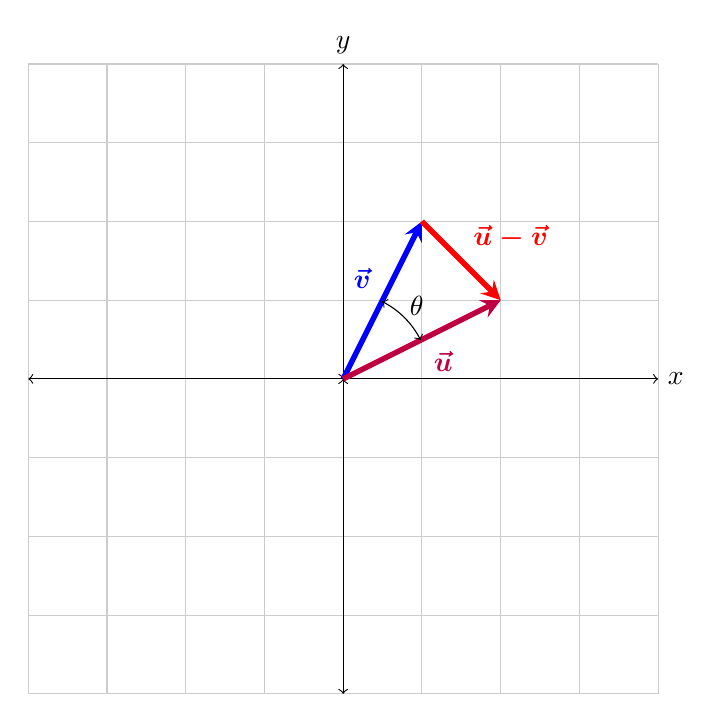
\begin{tikzpicture}
  \draw[thin,gray!40] (-4,-4) coordinate (o) grid (4,4);
  \draw[<->] (0,0)--(0,0) coordinate (o) node[right]{};
  \draw[<->] (-4,0)--(4,0)  node[right]{$x$};
  \draw[<->] (0,-4)--(0,4)  node[above]{$y$};
  \draw[line width=2pt,blue,-stealth](0,0)--(1,2) coordinate (x) node[midway,auto]{$\boldsymbol{\vec{v}}$};
  \draw[line width=2pt,purple,-stealth](0,0)--(2,1) coordinate (y) node[midway,auto,swap]{$\boldsymbol{\vec{u}}$};
  \draw[line width=2pt,red,-stealth](1,2)--(2,1) node[midway,auto]{$\boldsymbol{\vec{u}-\vec{v}}$};
 \pic [draw, <->,
      angle radius=11mm, angle eccentricity=1.2,
      "$\theta$"] {angle = y--o--x};
\end{tikzpicture}\\
$\mid\vec{u}-\vec{v}\mid^{2} = \mid\vec{u}\mid^{2} + \mid\vec{v}\mid^{2}-\hspace{.1cm}2\mid\vec{u}\mid\cdot\mid\vec{v}\mid\cos(\theta)$\\
\\
$\cancel{\mid\vec{u}\mid^{2}}-\hspace{.1cm}2\vec{v}\cdot\vec{u}\hspace{.1cm}+\cancel{\mid\vec{v}\mid^{2}}=\cancel{\mid\vec{u}\mid^{2}} + \cancel{\mid\vec{v}\mid^{2}}-2\mid\vec{u}\mid\cdot\mid\vec{v}\mid\cos(\theta)$\\
\\
$\cancel{-2}\vec{v}\cdot\vec{u} = \cancel{-2}\mid\vec{u}\mid\cdot\mid\vec{v}\mid\cos(\theta)$\\
\\
$\vec{v}\cdot\vec{u} = \mid\vec{u}\mid\cdot\mid\vec{v}\mid\cos(\theta)$\\
\end{enumerate}
\end{document}